\begin{block}{Experimental setup}
  Unique Ti:Sapphire pumped mode-locked laser system which allows orthogonal control of repetition rate $\Delta$ and offset freqency $\delta$. More details discussed in W-Y~Cheng,~\emph{et. al.} Appl. Phys. B, 92, 13-18(2008).
  \begin{figure}
    \begin{center}
      \setlength\fboxsep{0pt}
      \setlength\fboxrule{0.5pt}
      \fbox{\includegraphics[width=.9\linewidth]{figures/experiment_big}}
       % \includegraphics[width=.9\linewidth]{figures/experiment_big}
    \end{center}
    \label{Schematic of the experimental setup}
  \end{figure}
  W: output wedge, BS: beam splitter, CTSDL: cesium two-photon stabilized diode laser, DG: diffraction grating, SLM: spatial light modulator, AOM acousto-optic modulator, C: mechanical chopper, PMT: photo-multiplier tube
  \begin{itemize}
  \item The repetition rate $f_{rep}$ is near integer fraction of the ground-state splitting (e.g. 1/100 $\approx$ 92 MHz )
  \item Repetition rate locked to 5th harmonic of synthetizer (with 10~mHz stability)
  \item Time-base locked to LORAN-C signal
  \item SLM band pass filter bandwith $\approx$ 0.2 nm ($\approx$ 1 ps pulse length)
  \item Chopping frequency 500-1000 Hz
  \item Time-average input intensity 140$\mu$W with $<$1$\mu$W stability
  \end{itemize}
\end{block}
